\section{Transformação \texorpdfstring{$ Y-\Delta $}{Y-Δ}}

\frame{
	\frametitle{Introdução}
	\begin{block}{Definição}
		A transformação $Y-\Delta$, também chamada \textbf{delta-estrela}, delta-Y, estrela-triângulo, ou ainda, \textbf{Teorema de Kennelly}, é uma técnica matemática usada para \textbf{simplificar a análise de circuitos elétricos}.
	\end{block}
}

\frame{
	\frametitle{Introdução}
	\begin{block}{Motivação}
		Em certas configurações de circuitos, os resistores não parecem estar em \textbf{série} ou \textbf{paralelo}. Nestas condições, pode ser interessante \textbf{converter} o circuito de uma maneira para outra mais conveniente para determinar os valores das tensões e correntes. Duas configurações responsáveis por essas dificuldades são \textbf{estrela} ($Y$) e \textbf{triângulo} ($\Delta$)
	\end{block}
}

\frame{
	\frametitle{Introdução}
	
	\centering
	\begin{circuitikz}
		\draw (0,0) to[battery,l_=\SI{24}{\volt}] ++(0,2.2)
		-- ++(2,0)
		-- ++(0,-0.1)
		to[R=150<\ohm>,l=$ R_1 $, *-*] ++(-1,-1)
		to[R=100<\ohm>,l=$ R_3 $] ++(2,0)
		to[R=50<\ohm>,l=$ R_2 $] ++(-1,1) ++(-1,-1)
		to[R=300<\ohm>,l=$ R_4 $] ++(1,-1)
		to[R=250<\ohm>,l=$ R_5 $, *-*] ++(1,1) ++(-1,-1)
		-- ++(0,-0.1)
		-- ++(-2,0);
	\end{circuitikz}
	
%	\centerline{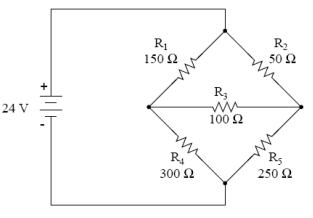
\includegraphics[width=0.6\linewidth]{Figuras/Ch01/fig1.jpg}}
	\begin{block}{Motivação}
		Como estão associados os resistores no circuito acima? Em série ou em paralelo? Como encontrar a \textbf{resistência equivalente} desse circuito?
	\end{block}
}

\frame{
	\frametitle{Rede estrela ($Y$)}
	
	\begin{minipage}{0.49\linewidth}
		\centering
		\begin{circuitikz}
			\draw (0,0) to[R,l_=$ R_1 $, o-*] ++(-30:1)
			to[R,l_=$ R_2 $, -o] ++(30:1) ++(30:-1)
			to[R=$ R_3 $, -*] ++(0,-1) ++(-0.5,0) to[short, o-o] ++(1,0);
		\end{circuitikz}\tikzmark{p1}
	\end{minipage}
	\hfill
	\begin{minipage}{0.49\linewidth}
		\centering
		\begin{circuitikz}
			\draw (0,0) to[R=$ R_1 $, o-*] ++(1,0)
			to[R=$ R_2 $, -o] ++(1,0) ++(-1,0)
			to[R=$ R_3 $] ++(0,-1) ++(-0.5,0) to[short, o-o] ++(1,0);
		\end{circuitikz}
	\end{minipage}

	\begin{tikzpicture}[remember picture, overlay]
		\draw[Implies-Implies, double distance=0.2cm,thick] (p1) ++(0,1.6cm) -- +(1,0);
	\end{tikzpicture}
	
%	\centerline{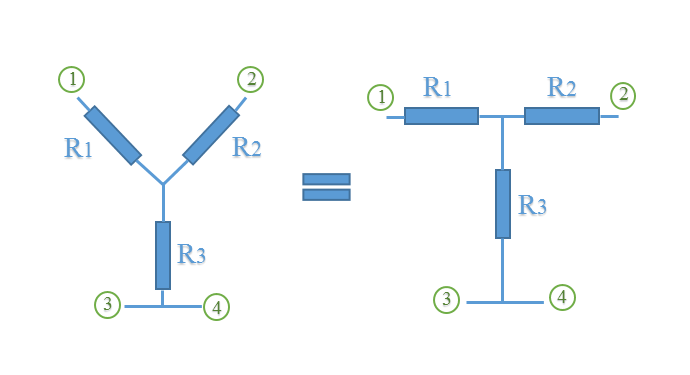
\includegraphics[width=0.9\linewidth]{Figuras/Ch01/fig2.png}}
}

\frame{
	\frametitle{Rede triângulo ($\Delta$)}
	
	\begin{minipage}{0.49\linewidth}
		\centering
		\begin{circuitikz}
			\draw (0.25,0) node[coordinate,name=a] {} ++(-30:1) node[coordinate,name=center] {}
			++(30:1) node[coordinate,name=b] {} ++(30:-1)
			++(0,-1) node[coordinate,name=c] {};
			\draw (0,0) to[short,o-] (a) to[R=$ R_c $] (b) to[short,-o] ++(0.25,0) (b)
			to[R,l^=$ R_a $, *-*] (c) (a)
			to[R,l_=$ R_b $, *-] (c) ++(-0.5,0) to[short, o-o] ++(1,0);
		\end{circuitikz}\tikzmark{p1}
	\end{minipage}
	\hfill
	\begin{minipage}{0.49\linewidth}
		\centering
		\begin{circuitikz}
			\draw (0.25,0) node[coordinate,name=a] {} ++(-30:1) node[coordinate,name=center] {}
			++(30:1) node[coordinate,name=b] {} ++(30:-1)
			++(0,-1) node[coordinate,name=c] {};
			\draw (0,0) to[short,o-] (a) to[R=$ R_c $] (b) to[short,-o] ++(0.25,0) (b)
			to[R,l^=$ R_a $, *-*] (b|-c) (a)
			to[R,l_=$ R_b $, *-*] (a|-c) ++(-0.25,0) to[short, o-o] ($ (b|-c)+(0.25,0) $);
		\end{circuitikz}
	\end{minipage}
	
	\begin{tikzpicture}[remember picture, overlay]
	\draw[Implies-Implies, double distance=0.15cm,thick] (p1) ++(-0.3,1.3cm) -- +(0.8,0);
	\end{tikzpicture}
	
%	\centerline{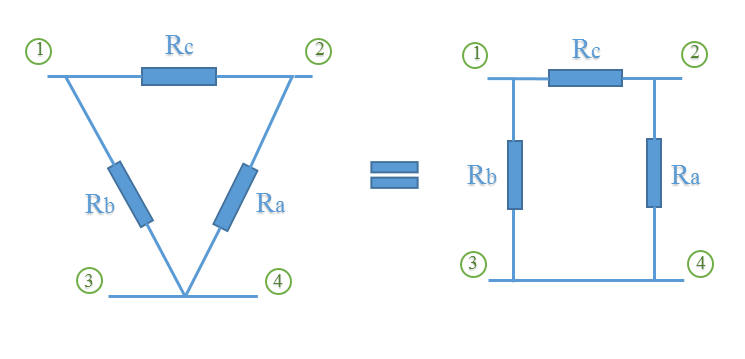
\includegraphics[width=0.9\linewidth]{Figuras/Ch01/fig3.png}}
}

\frame{
	\frametitle{Conversão $Y-\Delta$}
	\centering
	\begin{circuitikz}
		\draw[color=red] (0,0) node[coordinate,name=a] {} to[R,l_=$ R_1 $, o-*] ++(-30:1.5) node[coordinate,name=center] {}
		to[R,l_=$ R_2 $, -o] ++(30:1.5) node[coordinate,name=b] {} ++(30:-1.5)
		to[R=$ R_3 $, -*] ++(0,-1.5) node[coordinate,name=c] {} ++(-0.75,0);
		\draw[color=blue] (0,0) -- (a) to[R=$ R_c $, o-o] (b)
		to[R,l^=$ R_a $, *-*] (c) (a)
		to[R,l_=$ R_b $, *-] (c);
	\end{circuitikz}

	\begin{block}{Superposição}
		Observe o modelo de superposição das duas estruturas. Esse modelo ajuda a identificar a \textbf{conversão de uma rede para a outra}.
	\end{block}
}

\frame{
	\frametitle{Conversão $Y-\Delta$}
	\begin{block}{Terminais $1,3$}
		\textbf{Para o circuito em triângulo:}
		
		$$R_{1,3} = R_b \parallel (R_a + R_c) = \dfrac{R_b \cdot (R_a + R_c)}{R_b + R_a + R_c}$$
		
		\vspace{0.5cm}
		
		\textbf{Para o circuito em estrela:}
		
		$$R_{1,3} = R_1 + R_3$$
	\end{block}
}

\frame{
	\frametitle{Conversão $Y-\Delta$}
	\begin{block}{Terminais $1,2$}
		\textbf{Para o circuito em triângulo:}
		
		$$R_{1,2} = R_c \parallel (R_a + R_b) = \dfrac{R_c \cdot (R_a + R_b)}{R_c + R_a + R_b}$$
		
		\vspace{0.5cm}
		
		\textbf{Para o circuito em estrela:}
		
		$$R_{1,2} = R_1 + R_2$$
	\end{block}
}

\frame{
	\frametitle{Conversão $Y-\Delta$}
	\begin{block}{Terminais $2,4$}
		\textbf{Para o circuito em triângulo:}
		
		$$R_{2,4} = R_a \parallel (R_b + R_c) = \dfrac{R_a \cdot (R_b + R_c)}{R_a + R_b + R_c}$$
		
		\vspace{0.5cm}
		
		\textbf{Para o circuito em estrela:}
		
		$$R_{2,4} = R_2 + R_3$$
	\end{block}
}

\frame{
	\frametitle{Conversão $Y-\Delta$}
	\begin{block}{Importante}
		\begin{itemize}
			\item Quando sobrepomos um circuito em estrela a um circuito em triângulo, a resistência equivalente entre os terminais \textbf{deverá ser a mesma tanto para estrela, quanto para triângulo}. Deste modo:
		\end{itemize}
	
		\begin{gather}
		R_1 + R_3 = \dfrac{R_b \cdot (R_a + R_c)}{R_b + R_a + R_c} \label{eqn:1}\\
		R_1 + R_2 = \dfrac{R_c \cdot (R_a + R_b)}{R_c + R_a + R_b} \label{eqn:2}\\
		R_2 + R_3 = \dfrac{R_a \cdot (R_b + R_c)}{R_a + R_b + R_c} \label{eqn:3}
		\end{gather}

	\end{block}
}

\frame{
	\frametitle{Conversão $Y-\Delta$}
	\begin{block}{Obtenção das fórmulas}
		Subtraindo a equação \ref{eqn:3} da equação \ref{eqn:1}, obtemos:
		
		\begin{align}
			(R_2 + R_3) - (R_1 + R_3) &= \dfrac{R_a \cdot (R_b + R_c)}{R_a + R_b + R_c} - \dfrac{R_b \cdot (R_a + R_c)}{R_b + R_a + R_c} \nonumber\\
			R_2 - R_1 &= \dfrac{R_a \cdot R_b + R_a \cdot R_c - R_b \cdot R_a - R_b \cdot R_c}{R_b + R_a + R_c} \nonumber\\
			R_2 - R_1 &= \dfrac{R_a \cdot R_c - R_b \cdot R_c}{R_b + R_a + R_c} \nonumber\\
			R_1 - R_2 &= \dfrac{R_c \cdot (R_b - R_a)}{R_b + R_a + R_c} \label{eqn:4}
		\end{align}

	\end{block}
}

\frame{
	\frametitle{Conversão $Y-\Delta$}
	\begin{block}{Obtenção das fórmulas}
		Somando a equação \ref{eqn:2} da equação \ref{eqn:4}, obtemos:

		\begin{align}
			2 \cdot R_1 &= \dfrac{R_c \cdot R_b - R_c \cdot R_a + R_c \cdot R_a + R_c \cdot R_b}{R_b + R_a + R_c} \nonumber\\
			\Aboxed{R_1 &= \dfrac{R_b \cdot R_c}{R_a + R_b + R_c}} \label{eqn:5}
		\end{align}
	\end{block}
}

\frame{
	\frametitle{Conversão $Y-\Delta$}
	\begin{block}{Obtenção das fórmulas}
		Subtraindo a equação \ref{eqn:4} da equação \ref{eqn:2}, obtemos:

		\begin{align}
			-2 \cdot R_2 &= \dfrac{R_c \cdot R_b - R_c \cdot R_a - R_c \cdot R_a - R_c \cdot R_b}{R_b + R_a + R_c}\nonumber\\
			\Aboxed{R_2 &= \dfrac{R_a \cdot R_c}{R_a + R_b + R_c}} \label{eqn:6}
		\end{align}
	\end{block}
}

\frame{
	\frametitle{Conversão $Y-\Delta$}
	\begin{block}{Obtenção das fórmulas}
		Subtraindo a equação \ref{eqn:5} da equação \ref{eqn:1}, obtemos:

		\begin{align}
			-R_3 &= \dfrac{R_c \cdot R_b - R_b \cdot R_a - R_b \cdot R_c}{R_b + R_a + R_c}\nonumber\\
			\Aboxed{R_3 &= \dfrac{R_a \cdot R_b}{R_a + R_b + R_c}} \label{eqn:7}
		\end{align}
	\end{block}
}

\frame{
	\frametitle{Conversão $Y-\Delta$}
	\begin{block}{Regra Geral}
		Cada resistor do circuito em estrela é o \textbf{produto dos resistores nos dois ramos adjacentes} do circuito em triângulo, \textbf{dividido pela soma dos três resistores} em triângulo.
	\end{block}
}

\frame{
	\frametitle{Exemplo de Conversão $Y-\Delta$}
	
	\centering
	\begin{circuitikz}[scale=0.5]
		\draw (0,0) node[above] {$ A $} to[R=20<\ohm>,*-*] +(-60:2) node[below] {$ B $}
		to[R=12<\ohm>] (60:-2) node[below] {$ C $}
		to[R=68<\ohm>, *-] +(60:2);
	\end{circuitikz}
	
%	\centerline{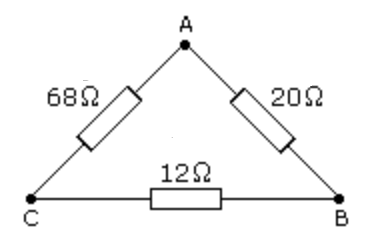
\includegraphics[width=0.3\linewidth]{Figuras/Ch01/fig5.PNG}}
	\begin{block}{Resolução}
		Resistores da rede $\Delta: R_a = 20 \si{\ohm}, R_b = 68 \si{\ohm}, R_c = \SI{12}{\ohm}$
		$$R_1 = \dfrac{R_b \cdot R_c}{R_a + R_b + R_c} = \dfrac{68 \cdot 12}{20 + 68 + 12} = \SI{8.16}{\ohm}$$
		$$R_2 = \dfrac{R_a \cdot R_c}{R_a + R_b + R_c} = \dfrac{20 \cdot 12}{20 + 68 + 12} = \SI{2.4}{\ohm}$$
		$$R_3 = \dfrac{R_a \cdot R_b}{R_a + R_b + R_c} = \dfrac{20 \cdot 68}{20 + 68 + 12} = \SI{13.6}{\ohm}$$
	\end{block}
}

\frame{
	\frametitle{Conversão $Y-\Delta$}
	\centering
	\begin{circuitikz}
		\draw[color=red] (0,0) node[coordinate,name=a] {} to[R,l_=$ R_1 $, o-*] ++(-30:1.5) node[coordinate,name=center] {}
		to[R,l_=$ R_2 $, -o] ++(30:1.5) node[coordinate,name=b] {} ++(30:-1.5)
		to[R=$ R_3 $, -*] ++(0,-1.5) node[coordinate,name=c] {} ++(-0.75,0);
		\draw[color=blue] (0,0) -- (a) to[R=$ R_c $, o-o] (b)
		to[R,l^=$ R_a $, *-*] (c) (a)
		to[R,l_=$ R_b $, *-] (c);
	\end{circuitikz}
%	\centerline{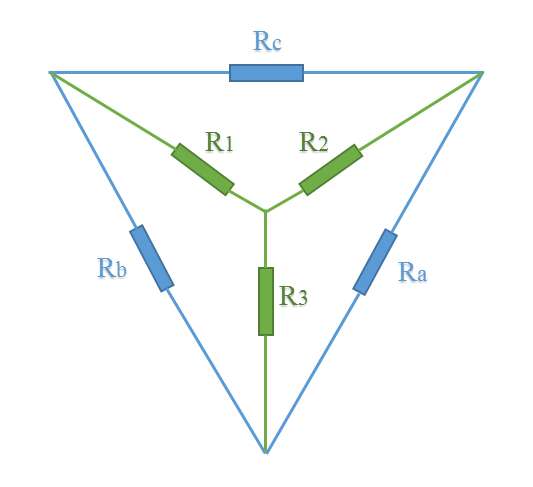
\includegraphics[width=0.5\linewidth]{Figuras/Ch01/fig4.png}}
	\begin{block}{Análogo}
		O princípio opara essa conversão é o mesmo para o circuito $\Delta-Y$, o que muda são as manipulações algébricas das equações.
	\end{block}
}

\frame{
	\frametitle{Conversão $Y-\Delta$}
	\begin{block}{Regra Geral}
		Cada resistor do circuito em triângulo é a \textbf{soma de todos os produtos possíveis dos resistores} do circuito em estrela tomados dois a dois, \textbf{dividido pelo resistor $\bm{Y}$ oposto}.

		\begin{equation*}
			\boxed{R_a = \dfrac{R_1 \cdot R_2 + R_1 \cdot R_3 + R_2 \cdot R_3}{R_1}}
		\end{equation*}
		\vspace{0.3cm}
		\begin{equation*}
			\boxed{R_b = \dfrac{R_1 \cdot R_2 + R_1 \cdot R_3 + R_2 \cdot R_3}{R_2}}
		\end{equation*}
		\vspace{0.3cm}
		\begin{equation*}
			\boxed{R_c = \dfrac{R_1 \cdot R_2 + R_1 \cdot R_3 + R_2 \cdot R_3}{R_3}}
		\end{equation*}
	\end{block}
}

\frame{
	\frametitle{Exemplo de Conversão $Y-\Delta$}
	
	\centering
	\begin{circuitikz}[scale=0.6, myR/.style = {R, resistors/scale=0.75, resistors/width=0.6, resistors/zigs=4}]
		\draw (0,0) node[above] {$ A $} to[myR,l=13.6<\ohm>, o-] ++(0,-1)
		to[myR,l_=8.16<\ohm>, *-o] ++(45:-1) node[below] {C} ++(45:1)
		to[myR,l=2.4<\ohm>, -o] ++(-45:1) node[below] {B};
	\end{circuitikz}
	
%	\centerline{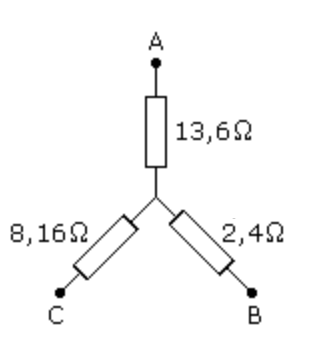
\includegraphics[width=0.22\linewidth]{Figuras/Ch01/fig6.PNG}}
	\begin{block}{Resolução}
		Resistores da rede $Y: R_1 = \SI{8.16}{\ohm}, R_2 = \SI{2.4}{\ohm}, R_3 = \SI{13.6}{\ohm}$
		$$R_a = \dfrac{R_1 \cdot R_2 + R_1 \cdot R_3 + R_2 \cdot R_3}{R_1} = \dfrac{\num{163,2}}{\num{8,16}} = \SI{20}{\ohm}$$
		$$R_b = \dfrac{R_1 \cdot R_2 + R_1 \cdot R_3 + R_2 \cdot R_3}{R_2} = \dfrac{\num{163,2}}{\num{2,4}} = \SI{68}{\ohm}$$
		$$R_c = \dfrac{R_1 \cdot R_2 + R_1 \cdot R_3 + R_2 \cdot R_3}{R_3} = \dfrac{\num{163,2}}{\num{13,6}} = \SI{12}{\ohm}$$
	\end{block}
}

\frame{
	\frametitle{Observação}
	\begin{block}{Rede equilibrada}
		As redes $Y$ e $\Delta$ são equilibradas quando:
		$$R_1 = R_2 = R_3 = R_Y \hspace{1.5cm} R_a = R_b = R_c = R_{\Delta}$$
		
		Logo,
		$$\boxed{R_Y = \dfrac{R_{\Delta}}{3}}$$
	\end{block}
}

\section*{Exercícios}
\frame{
	\frametitle{Exercícios}
	\begin{block}{}
		01. Encontre a resistência equivalente do circuito abaixo utilizando a transformação estrela-triângulo.
		
		\vspace{0.5cm}
		
		\centerline{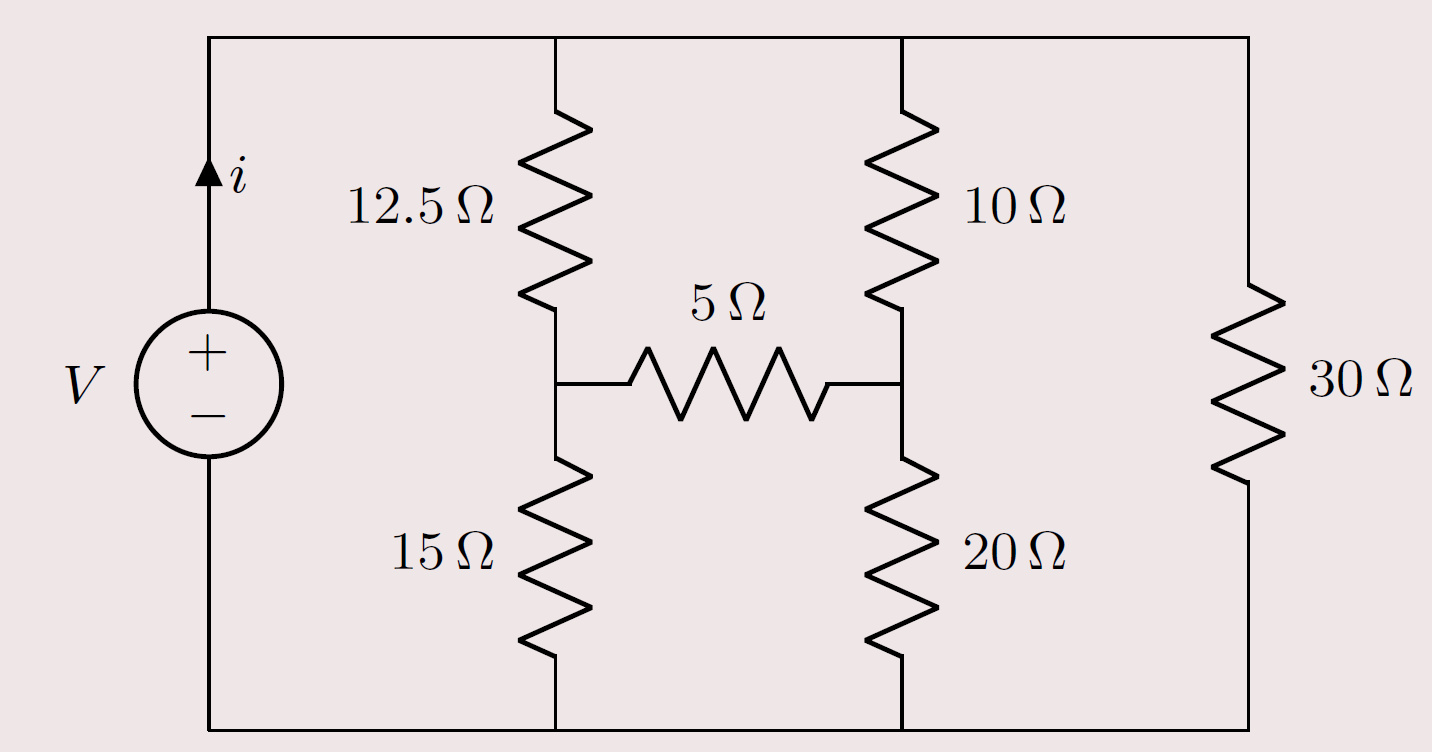
\includegraphics[width=0.6\linewidth]{Figuras/Ch01/fig7.PNG}}
	\end{block}
}

\section*{Referências}

\frame{
	\frametitle{Referências e Exercícios Complementares}
	\begin{itemize}
		\item ALEXANDRE, Charles K.; SADIKU, Matthew N. O. Fundamentos de Circuitos Elétricos. 5. ed. Porto Alegre: AMGH, 2013.
	\end{itemize}
	%\centering{\alert{Página 36 - \textbf{1.6.1 até 1.6.5, 1.6.17 até 1.6.19}}} \\
	\centering{\alert{Lista de exercícios 01}}
}